\documentclass[12pt,journal,compsoc]{IEEEtran}

\usepackage{graphicx}
\usepackage{caption}

\ifCLASSOPTIONcompsoc
\else
\fi
\ifCLASSINFOpdf

\else

\fi

\newcommand\MYhyperrefoptions{bookmarks=true,bookmarksnumbered=true,
pdfpagemode={UseOutlines},plainpages=false,pdfpagelabels=true,
colorlinks=true,linkcolor={black},citecolor={black},urlcolor={black},
pdftitle={Ceng435 - Term Project 1},
pdfsubject={Ceng435 - Term Project 1},
pdfauthor={Koray Can Yurtseven, Aykut Yardim},
pdfkeywords={Network, LaTeX, paper, template}}

\begin{document}

\title{Data Communications and Networking \\ Term Project 1}


\author{2099547 Koray Can Yurtseven | 2110278 Aykut Yardim}

\maketitle



\begin{abstract}
In this project we have designed a network which consists of a source node, a broker, 2 routers and a destination node. We have used Python programming language for implementing the design because of the flexibility of the language. We have sent data from the source node to destination node and measured delays between packets sent and concluded that packets are lost and the delay is increased  if the network becomes busy.
\end{abstract}

\section{Introduction}

\IEEEPARstart{I}{n} this project, we have designed a network which consists of a source node 's', a broker 'b', routers 'r1' and 'r2', and a destination node 'd'. We have used different connections between nodes. The connection between 's' and 'b' is a TCP connection. 'b' has 3 interfaces, the first is connected to the 's' and the other interfaces are connected to 'r1' and 'r2' respectively. Once the data comes to 'b' from 's' using TCP connection, it is stored to be packetized and it is forwarded to 'r1' and 'r2' using different interfaces and a UDP connection. After 'r1' and 'r2' are having the data, they send this data to the destination node 'd' using again UDP connections. Node 'd' has 2 interfaces. The node 'd' listens these interfaces and collects the data from them.\\
To calculate end to end delay, once the data is sent from the node 's', we have calculated the time-stamp and stored it in an array. To calculate end to end delay, we have synchronized 's' and 'd' and once the packet comes to the 'd', we calculated the arrival time of the packet and construct a packet for feedback mechanism. Then, this feedback packet is returned to the 's' using UDP connections between 's' to 'd'.\\
In this implementation, we have used Python programming language and took advantage of threads.\\
We have stored interfaces and port numbers for each connection in each file as global variables.

\section{Nodes}
In our project, we have used five different nodes for transferring data from source to destination. These are a source node 's', a broker 'b', two routers 'r1' and 'r2' and a destination node 'd'

\subsection{Source Node 's'}
In this node, we have deployed 2 python scripts. The first script named "creatorfilefor\_s" is used to create a file that is going to be sent over TCP connection. We have written different amounts of "1"'s to measure how different file size affects end to end delay and packet loss. Also we have read the file, because it is advised to do so since in the second term, we are going to transfer a file using the same topology.\\
Once the file creator script is run, then we can use "s.py" script to send the data over TCP connection.\\
In 's', we have a main function, which creates two threads which are responsible for sending the data over TCP connection and reading the data(time-stamps) over UDP connection. The main thread busy loops while the data is transmitting and there is no timeout.\\
The thread responsible for TCP connection reads file 98 byte per loop as a chunk data. We have chosen 98 byte per loop because once we read 98 bytes, we add the corresponding packet number for that loop and store both of them in JSON format which Storing the payload and  the packet number gives us 128 byte packet. To have always 128 byte packet, we have padded the packet number with zeros.\\
We have observed that, since the TCP sends the data back to back, the send times are very close to each other.\\
The other thread uses UDP connection to listen feedback packets from 'd'. When it receives a JSON packet, it serializes it and extract time information from it and stores in a global array.\\
Once everything is finished, main thread calculates average delay, print end to end delay times and joins threads.

\subsection{Broker Node 'b'}
In broker, we have implemented a TCP server, which listens its interface and port and serves request coming to this connection. We  could have used single TCP connection because the homework states that there will be only one connection to the broker, we have used general idea of handling TCP servers.\\
Once the TCP server receives a connection, it transfers this connection to a "udp\_service" to send the data to routers. Since TCP is byte oriented, we have to packetize our input. We have chosen our packet size as 128 byte and received bytes from TCP connection until we have received the desired amount of data or the connection is closed. After receiving the data packet, we have created 2 threads for each packet and send these packets to 'r1' and 'r2' using these threads.\\
We have also created 2 separate threads for listening feedback packets that comes from 'r1' and 'r2'. After receiving these feedback packets from routers, we have transmitted them to 's' using a UDP connection.

\subsection{Routers 'r1' and 'r2'}

In both routers, we have started two threads. Thread one is responsible for listening UDP connection for data coming from 'b' and forwards it to the destination 'd'. The second thread listens another socket which is connected to the 'd' for receiving feedback packets and once it receives those packets, it forwards it to broker 'b' using a UDP connection.

\subsection{Destination node 'd'}
In this node, we have created two threads for each UDP connection coming from routers. These threads are listening their connections to 'r1' and 'r2' separately and when the data comes, it prepares a packet which consists of received packet number and the current time-stamp. Then, it sends this feedback packet to the back where it comes from ('r1' or 'r2').

\section{End-to-end Delay Calculation}
As explained before, to calculate end to end delay, once we sent the data from 's', we have stored a time-stamp in 's'. After its feedback comes, we also stored feedback's time-stamp in a different array. After sending all the data and receiving all possible feedbacks, we calculated the difference between feedback packets' time-stamps and send data's time-stamps. Since the machines have different local times, we had difficulties to calculate differences. We used 'ntp' to synchronize these machines to the internet time using 'time.nist.gov' website.

\section{Results and Conclusions}

We have conducted 3 different experiments to calculate end to end delay with different scenarios. To simulate these experiments we have used 'netem' commands in unix to add different delays in each experiment. We have added the delays only to interfaces that are b to r1, b to r2, r1 to d, and r2 to d. We didn't add delays to interfaces that are in r1 to b, r2 to b, d to r1, and d to r2.\\
In the first experiment, we have added 1$\pm 5$ ms to each connection above and run our program 10 times to have average of these data. In the second and the third experiment, we have used 20$\pm 5$ms and 60$\pm 5$ms delays in interfaces respectively and calculated their average of 10 runs of our program.

\subsection{Average delay of a packet with size 128 byte experiment}

\begin{figure}[h!]
\centering
\captionsetup{justification=centering}
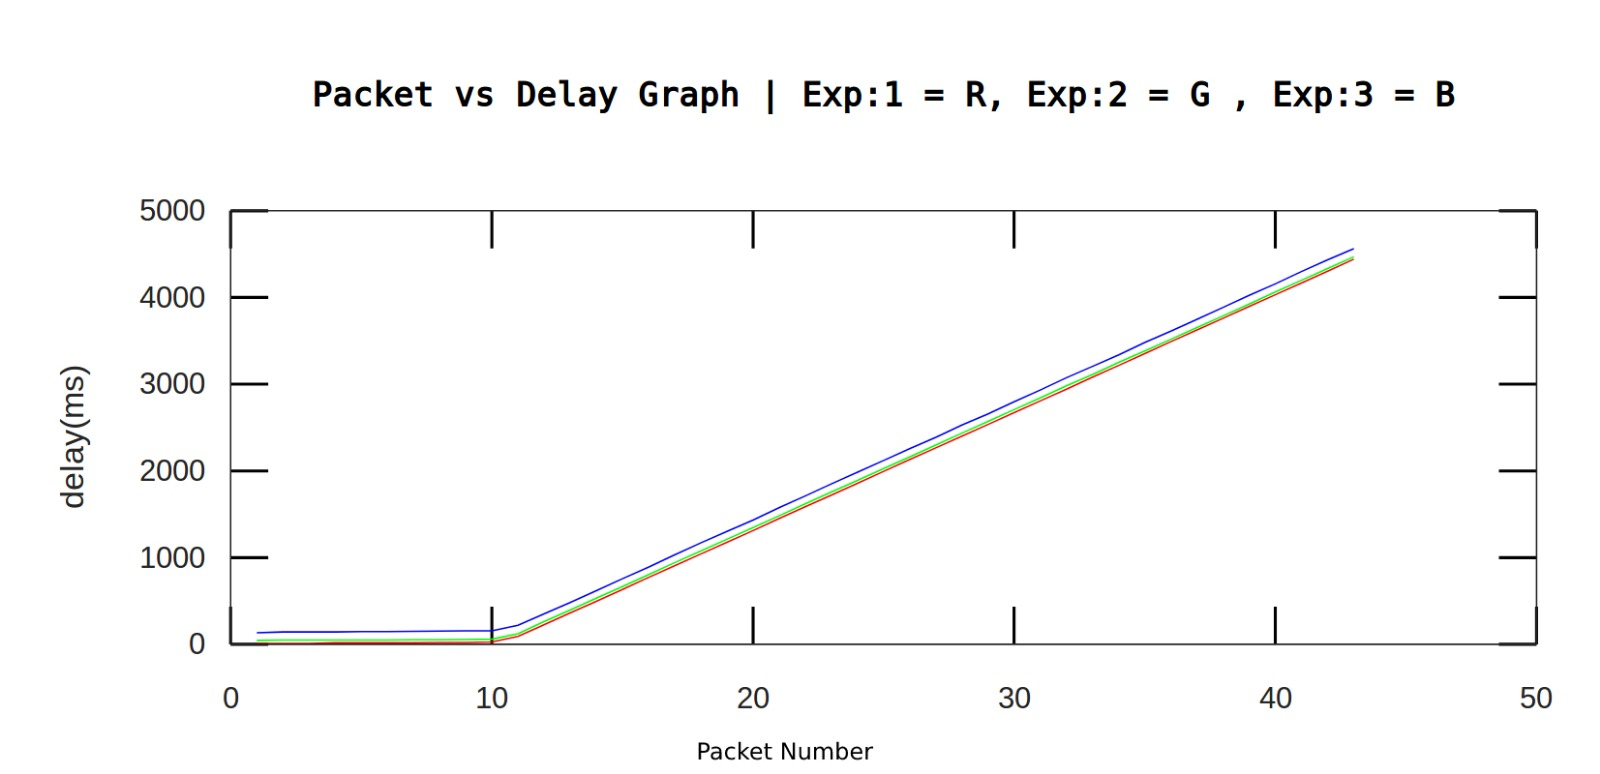
\includegraphics[width = \linewidth]{slope103.jpeg}
\caption{Packet vs Delay graphic}
\label{fig:slope103}
\end{figure}

As we can see in the Figure ~\ref{fig:slope103}, in three experiments, we observed similar results. These data are obtained from using differences between time-stamp of the feedback message and the time-stamp of the sent message which goes over the route s-b-r1-d. We didn't include the other route which is s-b-r2-d because we experienced similar results.\\
In the first experiment, using 1$\pm 5$ms delay in each node, the first ten packets delays are between 10 and 30. This is due to the fact that TCP sends the data very fast and since the network is not congested, these packets can arrive to the destination in short amount of time. However, after 10 packets, the delays are increasing and becomes 103ms in the average for a packet if we include the first 10 packets and becomes 131ms in the average for a packet if we exclude the first 10 packets. We have reached this result by calculating the slope of the line using the formula:
\begin{equation}
\label{eq:slopecalc}
 slope = \frac{\Delta increase\_in\_delay}{\Delta increase\_in\_packet\_number}
\end{equation}
After sending more than 40 packets,because of the network congestion and we have experienced packet loss.\\
In the second and the third experiment, we have experienced almost identical values, but the difference are the delays used. In the second and the third experiment, the first 10 data's end to end delay is larger than the first experiment by on the average 40ms and 120ms respectively. This is due the fact that we have added 20ms delay to 4 interface(b-r1, b-r2, r1-d, r2-d) in the second experiment, and 60ms delay in the third experiment.\\
In all of these three experiments, we have seen that average packet delay is 103ms by using formula (~\ref{eq:slopecalc}) after reaching some threshold which is 10 packets assuming that the packets are 128 byte. One can conclude that, the delay in interfaces changes the overall end to end delay but not the package's transmission delay which stays always 103ms.

\subsection{Total end to end delay experiment}
In this experiment, we again used three different delays as in the first experiment to measure total end to end delay for a given file.\\
\begin{figure}[h!]
\centering
\captionsetup{justification=centering}
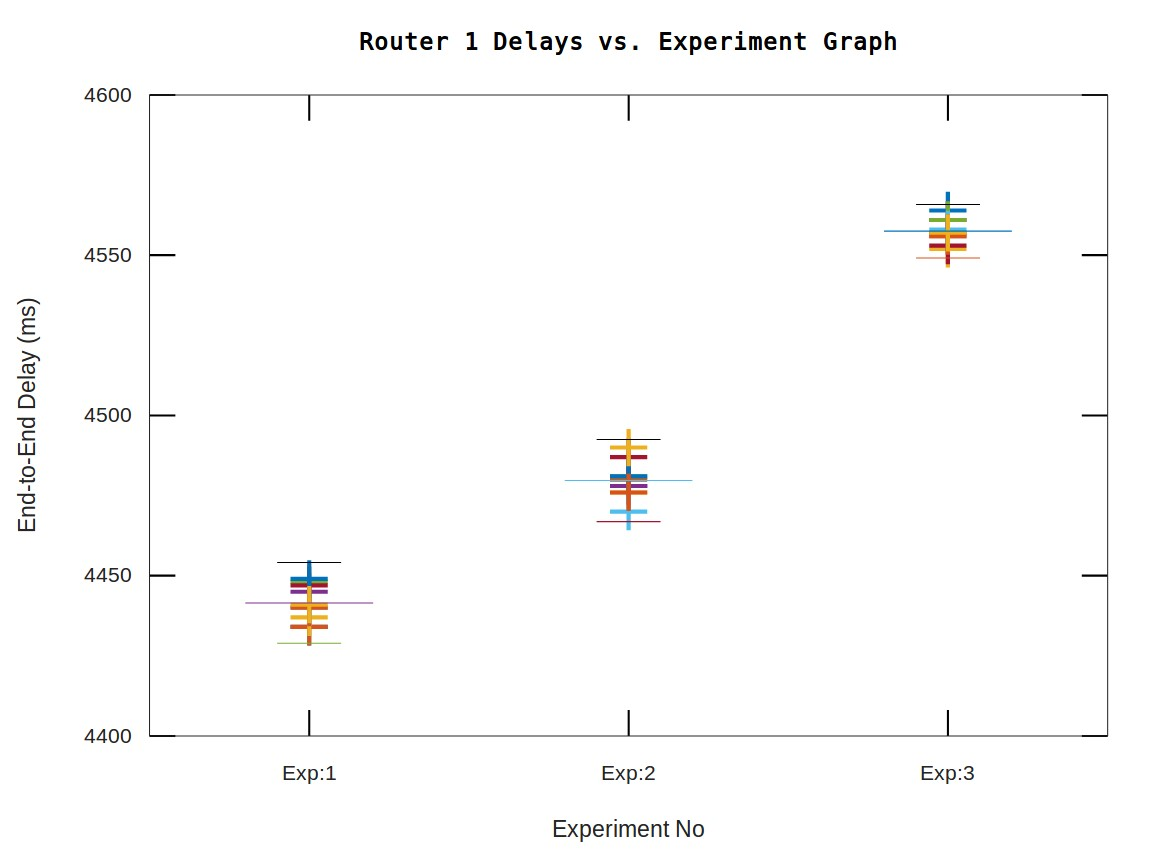
\includegraphics[width = \linewidth]{r1_confidence.jpeg}
\caption{End to end delay using router r1}
\label{fig:r1confidence}
\end{figure}
\begin{figure}[h!]
\centering
\captionsetup{justification=centering}
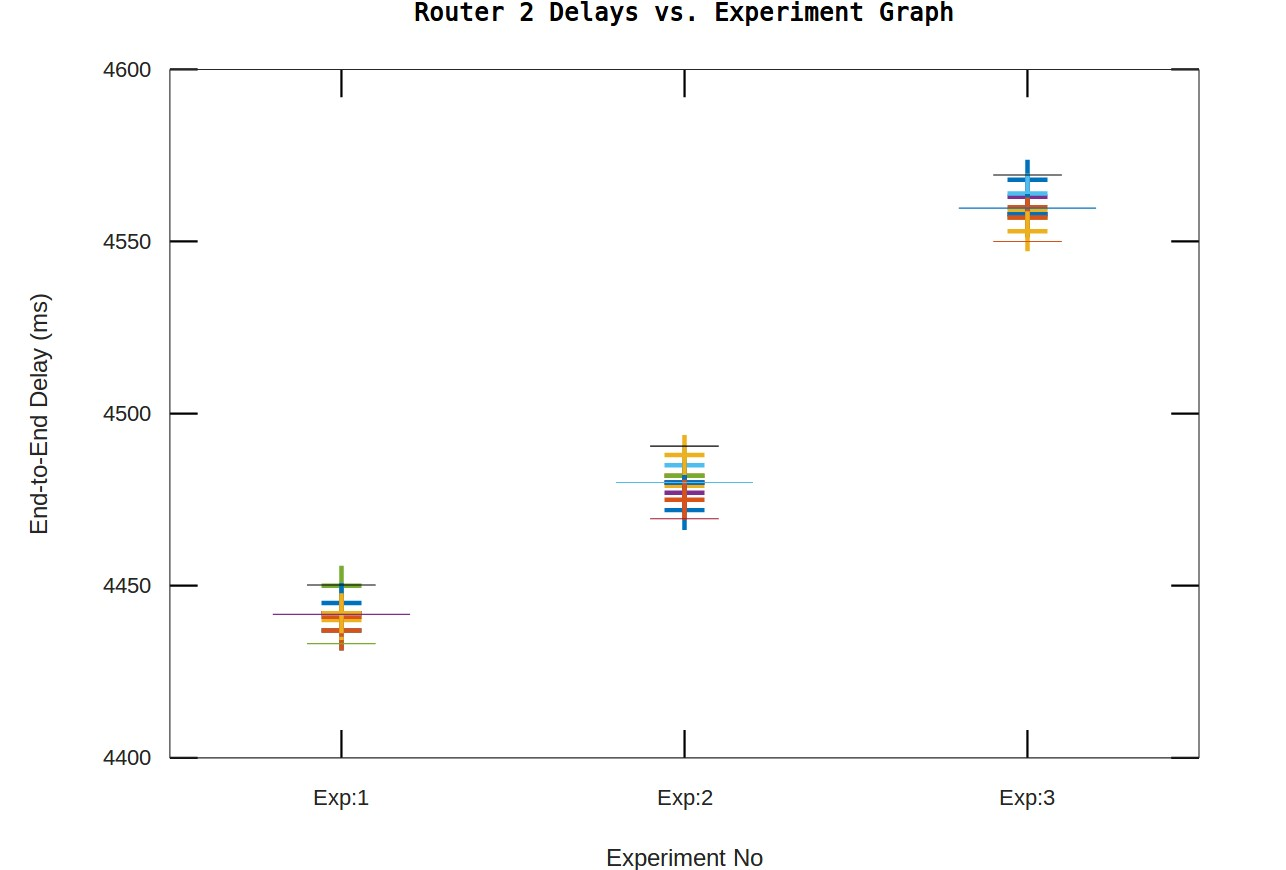
\includegraphics[width = \linewidth]{r2_confidence.jpeg}
\caption{End to end delay using router r2}
\label{fig:r2confidence}
\end{figure}

As we can see in the figure ~\ref{fig:r1confidence} and ~\ref{fig:r2confidence}, the end to end delay are almost the same. In the first figure, we measured total end to end delay in the route s-b-r1-d and in the second one using the route s-b-r2-d. Since we send all coming data to 'b' to the routers at the same time, they are equivalently busy. Thus, we measured same total end to end delay. Also, since we used UDP between 'b' and routers, and routers and 'd', we have experienced some packet loss.\\
We have run 3 experiment 10 times to get total end to end delay, and used that information to draw graphs above with 95\% confidence interval.\\

\begin{table}[h!]
\begin{tabular}{|l|l|l|l|}
\hline
              & Experiment 1 & Experiment 2 & Experiment 3 \\ \hline
R1 mean       & 4441         & 4480         & 4557         \\ \hline
R2 mean       & 4441         & 4480         & 4560         \\ \hline
R1 difference & -            & +39          & +116         \\ \hline
R2 difference & -            & +39          & +119         \\ \hline
Max R1        & 4449         & 4490         & 4561         \\ \hline
Min R1        & 4434         & 4470         & 4552         \\ \hline
Max R2        & 4450         & 4488         & 4564         \\ \hline
Min R2        & 4437         & 4475         & 4553         \\ \hline
\end{tabular}
\captionsetup{justification=centering}
\caption{Total End to end delay experiment results in ms}
\label{tab:e2eresults}
\end{table}

The data that we have used to calculate these values and plotting the figures are given in the appendixes A and B.\\

As a conclusion of the experiment, mean values can be estimated from total end to end delays.\\
Firstly, if we look at the r1 and r2 differences in the table, we can see that there are 39ms differences between experiment1 and experiment2, and there are 116ms and 119ms differences between experiment1 and experiment3. These mean difference values almost identical to the expected mean values which are 2*(20-1) = 38ms and 2*(60-1) = 118ms.\\
Secondly, if we look at the max and min values of r1 and r2 in the table above, we can see that it is in the range of $\pm 10$ms according to mean values. This is because we have used 2 different delays in the interfaces as stated previously.\\
Lastly, we can conclude the point that the delays are in the correct range, if we take the values for min r1 in the experiment1 and max r1 in the experiment3 or max r1 in the experiment1 and the min r1 in the experiment3. In the same way, it can also be examined using differences between experiment1 and experiment2, or using experiment2 and experiment3. As an example, we were expecting to have 78ms $\pm 20$ms difference between experiment2 and experiment3 using edge data which are max r1 for experiment2 and min r1 for experiment3. The difference between these two values is 4552 - 4490 = 62, which is in the correct range.

\appendices
\section{Fig2 data}

data = \\
4434 4478 4564;\\
4434 4480 4556;\\
4437 4476 4552;\\
4445 4478 4561;\\
4448 4481 4561;\\
4440 4470 4558;\\
4447 4487 4553;\\
4449 4481 4557;\\
4440 4476 4556;\\
4441 4490 4557




\section{Fig3 data}
data = \\
4437 4472 4568;\\
4437 4482 4560;\\
4440 4479 4559;\\
4442 4477 4563;\\
4450 4482 4557;\\
4441 4485 4564;\\
4442 4480 4558;\\
4445 4480 4558;\\
4441 4475 4557;\\
4442 4488 4553
\end{document}


